\begin{abstract}
We test whether spectral feedback on rotary-position attention gains improves
training-free 4K generation with FLUX.1-Krea-dev. Constancy RoPE compares the
predicted clean latent spectrum with a native-resolution reference and applies
a bounded, noise-gated correction to spatial attention gains. Two completed
campaigns fail to demonstrate an improvement over the released SEGA baseline.
In the second campaign, only SEGA plus time-matched constancy at gain $\eta=1$
passes the eight-prompt development gate. On 187 held-out prompt pairs, its
ImageReward difference is $+0.00857$ with a 95\% confidence interval of
$[-0.00841,0.02742]$, while full-resolution MUSIQ changes by $-0.20860$
$[-0.70887,0.31512]$. PickScore and crop MUSIQ decrease.
These results do not support an efficacy or state-of-the-art claim.
This working report records the completed experiments; it is not a
submission-ready methods paper.
\end{abstract}

\section{Question and tested controllers}
The project asks whether feedback toward a model's native latent spectrum can
improve resolution extrapolation through per-band attention gains. The target
image size is $4096\times4096$, compared with a $1024\times1024$ native
calibration size. The baseline is the released SEGA~\citep{sega2026} allocation and RoPE base,
identified in the implementation as \texttt{sega\_official}. The released
allocation differs from the paper-equation implementation; the two are not
interchangeable baselines.

The first campaign tested the original constancy controller, then a time-matched
native spectral target. The latter was also tested on SEGA's RoPE base with its
reference temperature. This did not establish an improvement. The second
campaign tested two effective-pool temperature rules, \texttt{alias\_temp}
and \texttt{alias\_temp\_sref}, and a composition of released SEGA with
time-matched constancy, \texttt{sega\_ctm}, at $\eta=0.5$ and $1.0$.

For the composed controller, let $m_d$ be SEGA's released query/key multiplier
for rotary pair $d$. A correction in spectral band $b$ is
\begin{align}
 e_b &= \tfrac12\bigl(\log P_{\mathrm{native},b}(\sigma)
              + a - \log \widehat P_b\bigr),\\
 \delta_b &= \eta w_b\,\clip(e_b,-1,1),\\
 g_d &= m_d^2\exp\bigl(\operatorname{interp}(\delta)_d\bigr).
\end{align}
Here $a$ is the anchor offset, $w_b$ is the existing visibility gate, and
$\widehat P_b$ is measured from the preceding transformer call's clean estimate.
The native target is interpolated at the current scheduler noise level.
Query and key are each multiplied by $m_d\exp(\delta_d/2)$.
The first step has no correction, the index axis retains unit gain, and no
additional global temperature is applied. Spectral powers use orthonormal
FFTs and means within bands. The vision analogy motivates this controller;
it does not establish its efficacy or novelty.

\section{What the gain algebra establishes}
\label{sec:audited-algebra}

\paragraph{Pair scaling and its causal limit.}
For fixed content vectors, the rotary-position logit~\citep{su2024roformer}
can be written as a finite trigonometric sum
\begin{equation}
 \ell(\Delta)=\frac{1}{\sqrt{d_k}}
 \sum_j \operatorname{Re}\bigl[c_j e^{i\theta_j\Delta}\bigr].
\end{equation}
Applying a shared multiplier $m_j$ to the query and key coordinates of pair $j$
multiplies that term by $m_j^2$. Its sign and phase still depend on $c_j$.
Increasing a high-frequency coefficient therefore does not by itself establish
more local attention, higher image-band power, or sharper decoded detail.
The three existing Krea development probes have inconsistent response signs:
one prompt has no positive decoded-width diagonal among six tested bands.
Those probes jointly perturb both spatial axes on NTK2, so they also cannot
identify a single-axis response under released SEGA.

\paragraph{Standardized profile shape.}
Let $\ell$ be a nonconstant vector of sampled log powers and let
$z(\ell)=(\ell-\operatorname{mean}\ell)/\operatorname{std}(\ell)$,
using one fixed standard-deviation convention. For $\beta>0$,
\begin{equation}
 z(a\mathbf{1}+\beta\ell)=z(\ell).
\end{equation}
This elementary identity applies to an ideal standardized-profile allocation.
It does not imply invariance of SEGA's radial spread or its complete gain.
The paper-inspired reference implementation adds a standard-deviation epsilon,
and the released implementation floors energy and standard deviation. Their
behavior is therefore invariant only under the corresponding inactive-floor
or negligible-stabilizer conditions, up to floating-point error. The statement
is about a formed log-power profile; raising a two-dimensional spectrum to a
power need not commute with averaging it into that profile.

\paragraph{Allocation and scalar magnitude are coupled.}
Before clipping, write a centered SEGA multiplier as
$m_j=m_{\mathrm{ref}}(1+a_j)$ with $\operatorname{mean}a_j=0$. Then
\begin{equation}
 \operatorname{mean}(m_j^2)
 =m_{\mathrm{ref}}^2\bigl[1+\operatorname{mean}(a_j^2)\bigr].
\end{equation}
Thus centering query/key multipliers does not preserve their mean squared
magnitude, which is the mean coefficient gain. Clipping changes these moments
again. The new RMS controls isolate this effect per spatial axis. They do not
match the actual attention-logit distribution, its variance, or its entropy.

\paragraph{Forward-noise expectation and the gate.}
For the linear data--noise interpolation used to motivate rectified
flow~\citep{liu2023flow}, assume independent data $x_0$ and unit white noise
$\varepsilon$, with $x_\sigma=(1-\sigma)x_0+\sigma\varepsilon$.
With an orthonormal transform, channel summation over $C$ channels, and
mean-per-band density on non-DC bands,
\begin{equation}
 \mathbb{E}_{\varepsilon} P_b(x_\sigma)
 =(1-\sigma)^2P_b(x_0)+\sigma^2C.
\end{equation}
The cross term vanishes in expectation. This is not an exact decomposition of
one noisy sample or one generated ODE trajectory. The controller's statistic
$\rho_b=\max(P_b(x_\sigma)/(\sigma^2C)-1,0)$ and gate
$w_b=\rho_b/(1+\rho_b)$ are design choices inspired by this identity. They do
not estimate the uncertainty of the delayed clean prediction. Likewise, zero
correction at an anchored target spectrum is an algebraic property of the
rule, not a stability theorem for the full sampling process.


\section{Executed protocol}
All reported comparisons use the FLUX.1-Krea-dev transformer with FLUX.1-dev
text encoders and VAE, $4096^2$ output, 28 sampling steps, distilled guidance
4.5, and scheduler shift $\mu=1.15$. The selected candidate and baseline share
the executed schedule, seed convention, and SEGA RoPE base. Earlier FLUX.1-dev
outputs exhibited a lattice artifact and are excluded from these results.

The 195 Aesthetic-4K evaluation captions are split into development rows 0--7
and held-out rows 8--194. Native calibration uses 16 separate Pick-a-Pic
prompts. Development eligibility requires positive mean differences in both
ImageReward and full-resolution MUSIQ, with CLIP difference at least $-0.3$.
At most two variants may advance; no settings change after selection.

The second campaign reports exactly 187 matched seed-0 prompt pairs. Generation
produced 188 images because row 7 was included to preserve task chunking; that
row is excluded from all held-out tables. Confidence intervals use 2,000 paired
bootstrap draws with bootstrap seed 0 and the 2.5 and 97.5 percentiles.
Intervals are nominal per metric, without multiple-comparison adjustment.
An interval crossing zero does not establish equivalence.

\section{Results}
\subsection{Development selection}
Table~\ref{tab:dev-current} records selection only. Both alias variants lose
ImageReward. The $\eta=0.5$ composition misses the MUSIQ gate by 0.007850.
Only $\eta=1$ advances; development scores are not generalization evidence.

\begin{table}[ht]
\centering\small
\setlength{\tabcolsep}{4pt}
\caption{Development means on eight prompts, seed 0.}
\label{tab:dev-current}
\begin{tabular}{@{}lrrrr@{}}
\toprule
Variant & ImageReward & MUSIQ & CLIP & Advance\\
\midrule
Released SEGA & 1.423018 & 42.488060 & 30.320004 & Reference\\
Alias temperature & 1.281098 & 35.807356 & 29.366986 & No\\
Alias, reference gain & 1.277426 & 44.972845 & 30.238460 & No\\
SEGA + constancy, $\eta=0.5$ & 1.441334 & 42.480210 & 30.200250 & No\\
SEGA + constancy, $\eta=1$ & 1.448742 & 42.505928 & 30.342451 & Yes\\
\bottomrule
\end{tabular}
\end{table}

\subsection{Held-out comparison}
\begin{table}[ht]
\centering\small
\caption{Held-out seed-0 means and paired differences, candidate minus released SEGA, over 187 prompts. Higher is better except the last three rows.}
\label{tab:heldout-current}
\begin{tabular}{@{}lrrr@{}}
\toprule
Metric & SEGA & SEGA + constancy & Difference [95\% CI]\\
\midrule
ImageReward & 1.18994 & 1.19852 & $+0.00857$ [$ -0.00841, +0.02742 $]\\
PickScore & 23.05255 & 22.97729 & $-0.07526$ [$ -0.10234, -0.04914 $]\\
CLIP & 29.13552 & 29.04160 & $-0.09392$ [$ -0.19651, -0.00368 $]\\
MUSIQ, full image & 45.22784 & 45.01924 & $-0.20860$ [$ -0.70887, +0.31512 $]\\
MUSIQ, 1024 crops & 58.32778 & 57.19612 & $-1.13166$ [$ -1.38754, -0.90219 $]\\
CLIP-IQA, full image & 0.60299 & 0.60593 & $+0.00294$ [$ -0.00018, +0.00609 $]\\
CLIP-IQA, 1024 crops & 0.58597 & 0.58846 & $+0.00250$ [$ -0.00070, +0.00563 $]\\
Spectrum log RMSE & 1.06838 & 1.06596 & $-0.00242$ [$ -0.00905, +0.00433 $]\\
Spectrum slope error & 0.19995 & 0.19741 & $-0.00254$ [$ -0.00678, +0.00192 $]\\
Tiling at 1024 & 0.06836 & 0.06844 & $+0.00008$ [$ -0.00072, +0.00081 $]\\
\bottomrule
\end{tabular}
\end{table}

The selected composition has no demonstrated gain on ImageReward or
full-resolution MUSIQ. PickScore, crop MUSIQ, and CLIP have negative nominal
confidence intervals. The remaining intervals cross zero. This second
campaign therefore does not repair the original controller's failure.

The earlier time-matched controller on SEGA's base also regresses on the same
187 seed-0 prompts. Full-resolution MUSIQ changes by $-3.03602$, with interval
$[-4.28169,-1.81488]$. Crop MUSIQ changes by $-2.19266$, with interval
$[-2.81241,-1.56666]$. Its ImageReward difference is unresolved at
$+0.01782$ $[-0.02271,0.05913]$. A temperature-only control on SEGA's base
reduces full-resolution MUSIQ by $2.08550$ points, with a paired interval
$[-3.24526,-0.96407]$. These comparisons constrain the tested designs;
they do not show that all spectral controllers must fail.

\begin{figure}[t]
\centering
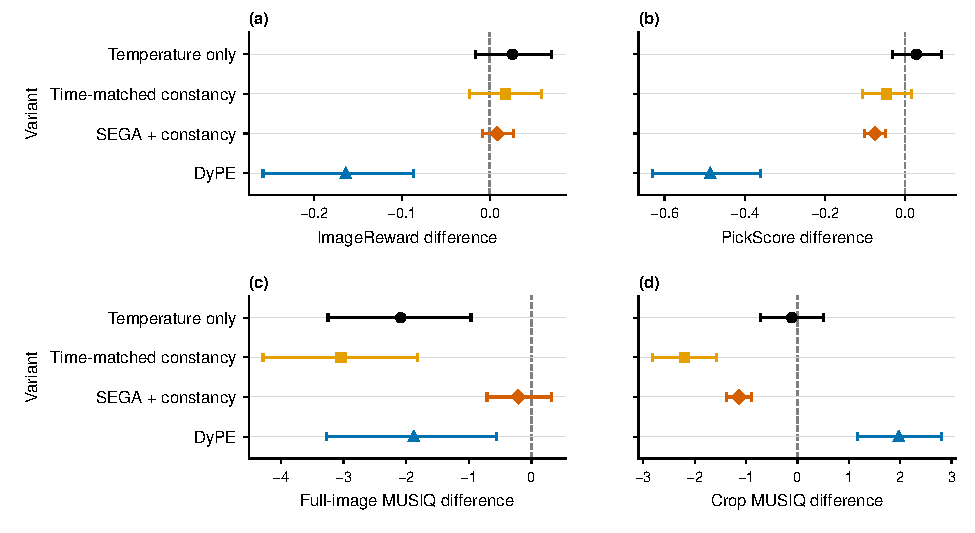
\includegraphics[width=\linewidth]{figs/heldout_comparison.pdf}
\caption{Neither constancy variant demonstrates a joint preference and quality
gain over released SEGA. Points show paired differences; whiskers are nominal
95\% prompt-bootstrap intervals from 2,000 draws over 187 prompts, single seed.
Zero is the released SEGA baseline; higher is better in all panels. DyPE's crop
quality gain accompanies a preference loss. The temperature-only and time-matched
constancy variants use SEGA's RoPE base and reference temperature.}
\label{fig:heldout-current}
\end{figure}

\begin{figure}[p]
\centering
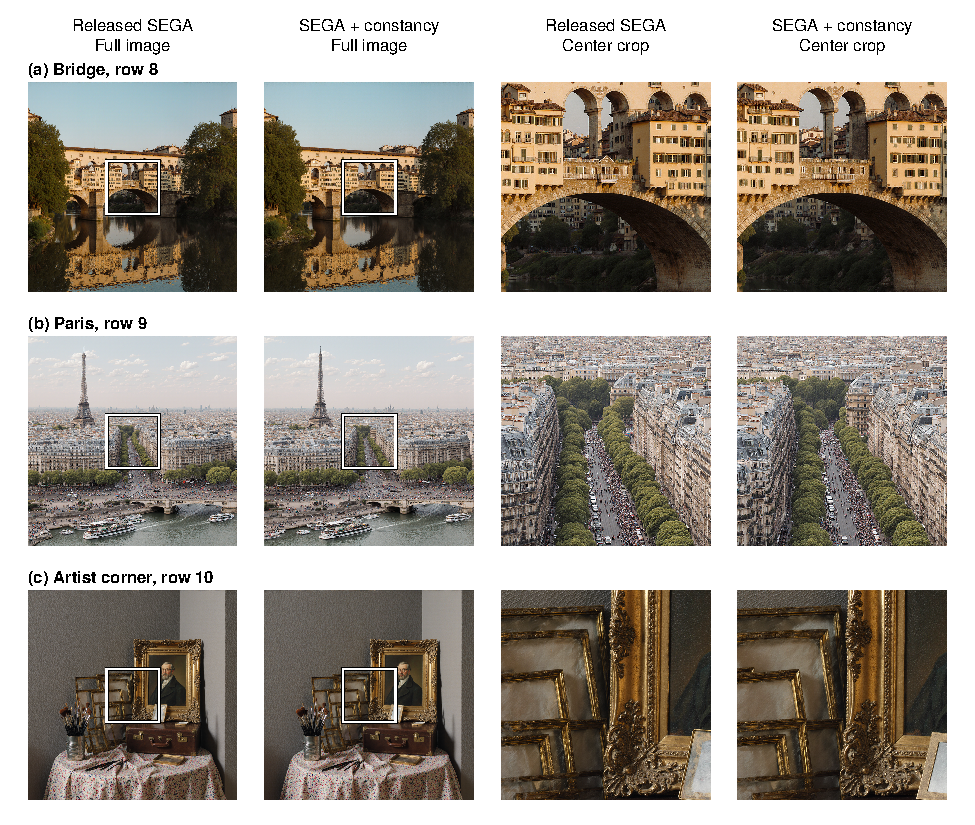
\includegraphics[width=\linewidth]{figs/heldout_examples.pdf}
\caption{Fixed-order examples from the completed second campaign: the first
three held-out captions, rows 8--10, seed 0. Columns compare released SEGA with
SEGA plus constancy at $\eta=1$, followed by their native $1024^2$ center crops.
Boxes show the crop coordinates in the $4096^2$ full outputs. The same pixel
coordinates are used in each image; generated content need not align exactly.
Full images are reduced for display, and crops receive no enhancement.
Rows were fixed before viewing these images and were not selected by scores.
Three examples cannot establish preference or quality differences; the paired
187-prompt measurements supply the quantitative evidence.}
\label{fig:heldout-examples}
\end{figure}

\section{Limits and continuation}
\paragraph{Novelty and current comparison scope.}
A successful continuation requires a distinct mechanism with competitive quality
and cost against recent resolution-extrapolation methods. Adaptive spectral gains
are already introduced by SEGA; temporal positional schedules by
DyPE~\citep{issachar2025dype}; entropy-based concentration by
UltraImage~\citep{ultraimage2025}; and text anchoring with dynamic temperature by
TIDE~\citep{tide2026}. HRDiT~\citep{hrdit2026} combines spatial position alignment
and head-adaptive pruning. More recently, AReA~\citep{area2026} changes attention
from coarse cross-scale to progressively local receptive fields, while Spectral
Correction Guidance~\citep{scg2026} corrects sampling toward a reference spectrum.
CSFlow~\citep{csflow2026} connects contrast sensitivity to flow-time weighting.
Thus spectral feedback, perceptual motivation, normalization, or a timing change
alone cannot establish the proposed contribution. The current RMS and timing
controls are diagnostics. The completed SEGA comparisons do not establish
competitiveness against this expanded set, and a development pass alone does not
justify promoting a control to a new method. No near-SOTA or SOTA claim follows
from the present evidence.

\paragraph{Local response diagnostic under development.}
The earlier octave interventions compare complete sampling trajectories, so they
do not identify a local map from attention gain to spectral power. A new diagnostic
replays a selected transformer state with identical latent, conditioning, and
noise level. It perturbs height and width gains separately while preserving the
affected axis's query/key RMS, alongside a spatial scalar control. Symmetric
finite differences estimate the response of the clean-estimate spectrum; smaller
perturbations check prediction accuracy. Only the baseline output advances the
sampler. CPU tests, including a small randomly initialized FLUX transformer, check
exact trajectory and state restoration. Pretrained GPU validation and response
measurements remain unrun. This is an instrument for testing the controller
hypothesis, not a new validated generation method. SCG acts directly on latent
Fourier magnitudes, whereas this diagnostic measures the response to internal
attention gains~\citep{scg2026,sega2026}; this difference alone does not establish
novelty or improved quality.

The second-campaign candidate has one held-out seed and one evaluated backbone
at one resolution. No second-seed replication of this candidate, new backbone,
human preference study, or broader resolution claim is supported. Aggregate
FID/KID scores from the raw 188-image evaluation include development row 7 and
are excluded from the held-out conclusion. No new throughput comparison is
claimed in this report.

The earlier extended theory and literature sections remain in the source tree
but are excluded because they describe superseded settings and unresolved claims.
Section~\ref{sec:audited-algebra} retains only qualified algebraic observations.
The third diagnostic below tests gain magnitude, frequency allocation, and
controller timing under a frozen development-only protocol. The already inspected held-out set must not become a
tuning set presented as fresh evaluation.

\IfFileExists{sec/dev3_results.tex}{\paragraph{Third development diagnostic.}
The three prespecified controls and a fresh released-SEGA baseline completed on eight development prompts, seed 0. These are exploratory selection scores, not held-out efficacy evidence.
\begin{table}[ht]
\centering\small
\setlength{\tabcolsep}{4pt}
\caption{Third development diagnostic. Differences are against the fresh same-hardware SEGA baseline.}
\begin{tabular}{@{}lrrrrl@{}}
\toprule
Variant & $\Delta$IR & $\Delta$MUSIQ & $\Delta$CLIP & $\Delta$crop MUSIQ & Gate\\
\midrule
RMS-matched uniform & -0.0174 & -1.5667 & +0.5868 & -0.5177 & Fail\\
RMS-normalized allocation & +0.0363 & +0.3889 & -0.0655 & -0.2150 & Pass\\
Lag-aligned constancy & +0.0193 & -0.2233 & +0.0092 & -0.1530 & Fail\\
\bottomrule
\end{tabular}
\end{table}
PickScore differences against the same baseline are RMS-matched uniform: -0.0832; RMS-normalized allocation: -0.0666; Lag-aligned constancy: -0.0546.
RMS-normalized allocation passed the development gate. These controls remain diagnostics, not an established novel method. A separate set of 64 confirmation captions was frozen before these outcomes; its use requires a distinct method and a recent-baseline protocol. No confirmation result or efficacy claim follows from this table.
}{%
\paragraph{Prespecified development diagnostics, not results.}
A third diagnostic compares three controls on development rows 0--7:
released-SEGA allocation normalized to the reference query/key RMS; spatially
uniform gains matched to the released allocation's realized RMS; and the
$\eta=1$ constancy composition with its target evaluated at the delayed
estimate's own scheduler noise level. A fresh released-SEGA run is the reference.
These distinguish gain magnitude from frequency allocation and isolate target
timing. The code passes 256 CPU tests, but no GPU outcome for these controls is
available in this snapshot. The planned job contains 32 images and was queued
on October 17. A positive development result remains diagnostic; advancing a
method requires a defensible novelty distinction and separate confirmation.
}

\paragraph{Conditional confirmation protocol.}
Before the third development outcome, a separate set of 64 captions was frozen
from Aesthetic-4K's 2048-source split after excluding normalized matches to all
prior evaluation and calibration captions. Fixed hash ordering selected the
captions without inspecting generation or scores. A candidate that satisfies
both the method-novelty review and a separately frozen development protocol would
use its unchanged settings at $4096^2$ with a fresh SEGA baseline. The captions
are fresh to this project's evaluation, with no model-training disjointness or
semantic-near-duplicate guarantee. They do not supply matched 4K reference images.
The prespecified analysis uses 10,000 paired prompt-bootstrap draws, seed 0,
and common resampling indices across metrics and candidates. Nominal 95\%
intervals accompany all metrics. For the two primary metrics, ImageReward and
full-image MUSIQ, Bonferroni-adjusted percentile intervals have coverage
$1-0.05/(2K)$ for $K$ selected candidates. Joint primary support requires both
adjusted lower bounds to exceed zero. These are approximate bootstrap intervals,
not exact finite-sample guarantees. Secondary losses remain part of the report;
confirmation cannot select further controller settings. No confirmation result
is available in this snapshot.

\paragraph{Evidence provenance.}
The completed campaign is recorded at implementation commit
\texttt{a1ede1a} on October 16, 2026. Its archived paired table, per-prompt
scores, and analysis protocol are in \path{.agent/notes/main2/}.
The current held-out table is generated from those CSVs after checking its
means and paired intervals against the per-prompt records. This check reuses
saved scorer outputs; it is not a fresh image-scoring reproduction.
The previous session records 194 passing CPU tests.
\IfFileExists{sec/dev3_results.tex}{The third diagnostic adds new inference and
evaluation; its development-only outcome is reported separately above.}{No new
inference or training result is included in this snapshot.}
